%%%%
\section{Fluorescência de Raios X}

Para determinação e quantificação das concentrações elemenares (número atômico $Z>10$)
foi utilizada a técnica não-destrutiva de \textit{Fluorescência de Raios X}.

\textit{Fluorescência de Raios X} é um método analítico quali-quantitativo, 
multielementar, que mede os raios-X característicos emitidos dos átomos da amostra, 
depois de também serem irradiados por Raios X. Não exige pré-tratamento químico
das amostras.

A figura \ref{fig:shimadzu_atomo} ilustra classicamente o que ocorre com
o átomo ao ser excitado.

\begin{figure}[H]
\begin{center} 
  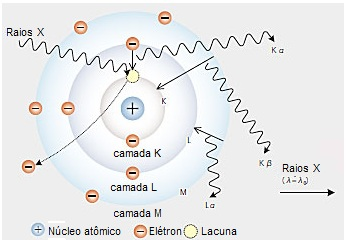
\includegraphics[width=0.5\textwidth]{../inputs/images/shimadzu_atomo.jpg}
  \caption{Shimadzu - Figura que acompanha o manual do XRF-ED \label{fig:shimadzu_atomo}}
   % http://www.shimadzu.com.br/analitica/produtos/elemental/raios_x/eds/images/edx-7000_8000-2.jpg
\end{center}
\end{figure}

O feixe de raios x incidente, neste caso produzido por tudo de raios X, 
expulsa os elétrons das camadas mais internas $K$ e $L$, produzindo 
"vazios", chamados de vacâncias. Um átomo com vacância é instável e
rapidamente elétrons das camadas mais externa preenchem  dfdf

As transições dos elétrons das camadas mais externas para as camadas
$K$ e $L$ liberam energias na região dos Raios X, que são características
do átomo em questão. 

Transições da camada $L$ para $K$ são do tipo $K\alpha$, de $M$ para $K$ 
são $K\beta$ e de $M$ para $L$ são $L\alpha$ ou $L\beta$. 
Apesar $K\alpha$  Algumas transições tem 
energias tão próximas que .


%TODO: Fazer diagrama das transições. Lembrando que há transições proíbidas. 

%%%%

O rendimento é calculado pelos raios X efetivamente emitidos em relação as 
vacâncias produzidas.

Existem 3 Tipos de fluorescências de raios X:
\begin{itemize}
  \item Dispersão de Energia;
  \item Dispersão de comprimento de onda;
  \item Reflexão total.
\end{itemize}


Outra forma de excitação usada é por partículas aceleradas 
(elétrons, prótons, íons, partícula alfa e beta negativa).

Amostra espessas apresentam o efeito matriz, ou seja, interações dos 
raios X característicos com os elementos da amostras, causando 
absorção do raios X ou mesmo reforço de raios X.


\subsection{Fluorescência de Raios X por dispersão em energia}

Os dispersivos em energia usam semicondutor capaz de discriminar energia 
próximas, onde a distinção dos fótons é feita pela amplitude do pulso 
eletrônico produzido no detector, já que os pulsos eletrônicos são
proporcionais às energias dos raios X. 

O detector mais empregado é o detector de silício ativado com lítio, Si(Li).

\subsection{Formulação Matemática}

Energia de ligação pode ser aproximada pela teoria atômica de Bohr:
\begin{math}
E = \frac{me^4(Z-b)^2}{8w^2h^2n^2}
\end{math}

\begin{itemize}
  \item E = energia de ligação eletrônica (joules);
  \item m = massa de repouso do elétron = 9,11.10 -31 kilogramas;
  \item e = carga elétrica do elétron = 1,6.10 -19 coulombs;
  \item Z = número atômico do elemento emissor dos raios X;
  \item b = constante de Moseley, com valores iguais a 1 e 7,4, 
        para as camadas K e L, respectivamente;
  \item w = o = permitividade elétrica no vácuo = 8,8534.10 -12 
        coulombs.newton -l .metro -2;
  \item h = constante de Planck = 6,625.10 -34 joules.s;
  \item n = n o quântico principal do nível eletrônico 
        (n = 1 para camada K, n = 2 para camada L, etc.).
\end{itemize}

%%%%
\subsection{Limite de Detecção}

Densidade mínima para haver detecção da espécie. % como determina para XRF?

\begin{figure}[H]
\begin{center}
  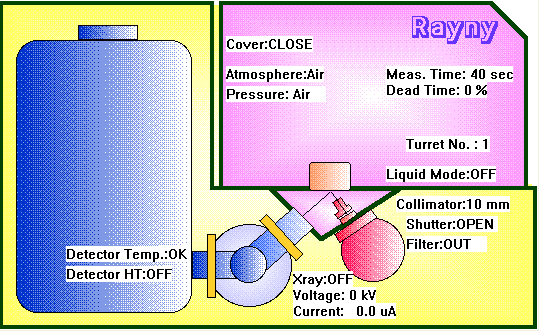
\includegraphics[scale=0.4]{../inputs/images/edx_iag_monitor.png}
  \caption{edx}
\end{center}
\end{figure}



